\subsection{Tutorial: De Descenso de Gradiente a Familias de Optimizadores}
\label{sec:opt-tutorial}

El resto de este apéndice es una referencia: una entrada por optimizador, con
su regla de actualización, su pseudocódigo y su perfil de memoria. Esta
subsección es la rampa de entrada. Presenta las cinco ideas que toda entrada
reutiliza---la superficie de pérdida, el gradiente, el tamaño de paso, el lote
y los dos estadísticos que añaden los métodos posteriores---y después compara
las familias como familias, sin derivar ningún método concreto. Quien la
termine debería poder abrir cualquiera de las secciones siguientes y reconocer
cuál de las cinco ideas está modificando.

\subsubsection{Un problema, muchas recetas}
\label{sec:opt-tutorial-problem}

Entrenar una red neuronal es un problema de optimización envuelto en
contabilidad. Sea $\theta$ el vector de todos los números entrenables (pesos y
sesgos, decenas de millones para un transformer pequeño), $L(\theta)$ la
pérdida y $f(\theta)$ el objetivo que realmente se minimiza, normalmente $L$
más un regularizador. La arquitectura solo decide \emph{cuál} es la superficie
$L$: el número de capas, el patrón de atención, la normalización, la
activación. El optimizador decide \emph{cómo avanza el recorrido} sobre esa
superficie. Todo optimizador de este apéndice se puede escribir en una línea,
\begin{equation}
\theta_{t+1} \;=\; \theta_t \;-\; \eta_t\, u_t,
\qquad u_t = u\!\left(g_t, g_{t-1}, \dots,\, \theta_t\right),
\label{eq:opt-tut-generic}
\end{equation}
donde $g_t=\nabla f(\theta_t)$ es el gradiente y $u_t$ es una dirección
construida a partir del gradiente actual y, quizá, de una pequeña cantidad de
estado recordado. El descenso de gradiente toma $u_t=g_t$. Momentum toma $u_t$
como un promedio decreciente de gradientes pasados. Los métodos adaptativos
dividen $u_t$ coordenada a coordenada. Los métodos de segundo orden lo rotan
con una estimación de la curvatura. Los métodos de ortogonalidad le dan forma
de matriz. Nada más cambia: el signo delante de $\eta_t$ es siempre negativo,
porque el gradiente apunta cuesta arriba.

La imagen habitual es la de un excursionista que baja una montaña con niebla
\citep{ibm_sgd_2025}. Siente la pendiente bajo sus pies pero no ve el valle, así
que la estrategia se reduce a tres preguntas: cuán fiable es la lectura de la
pendiente (¿un ejemplo o mil?), cuán larga es la zancada y cuánta memoria del
terreno merece la pena cargar. La Figura~\ref{fig:opt-tut-flow} convierte esas
preguntas en el mapa de las familias que siguen.

\begin{figure}[H]
\centering
\fitfigure{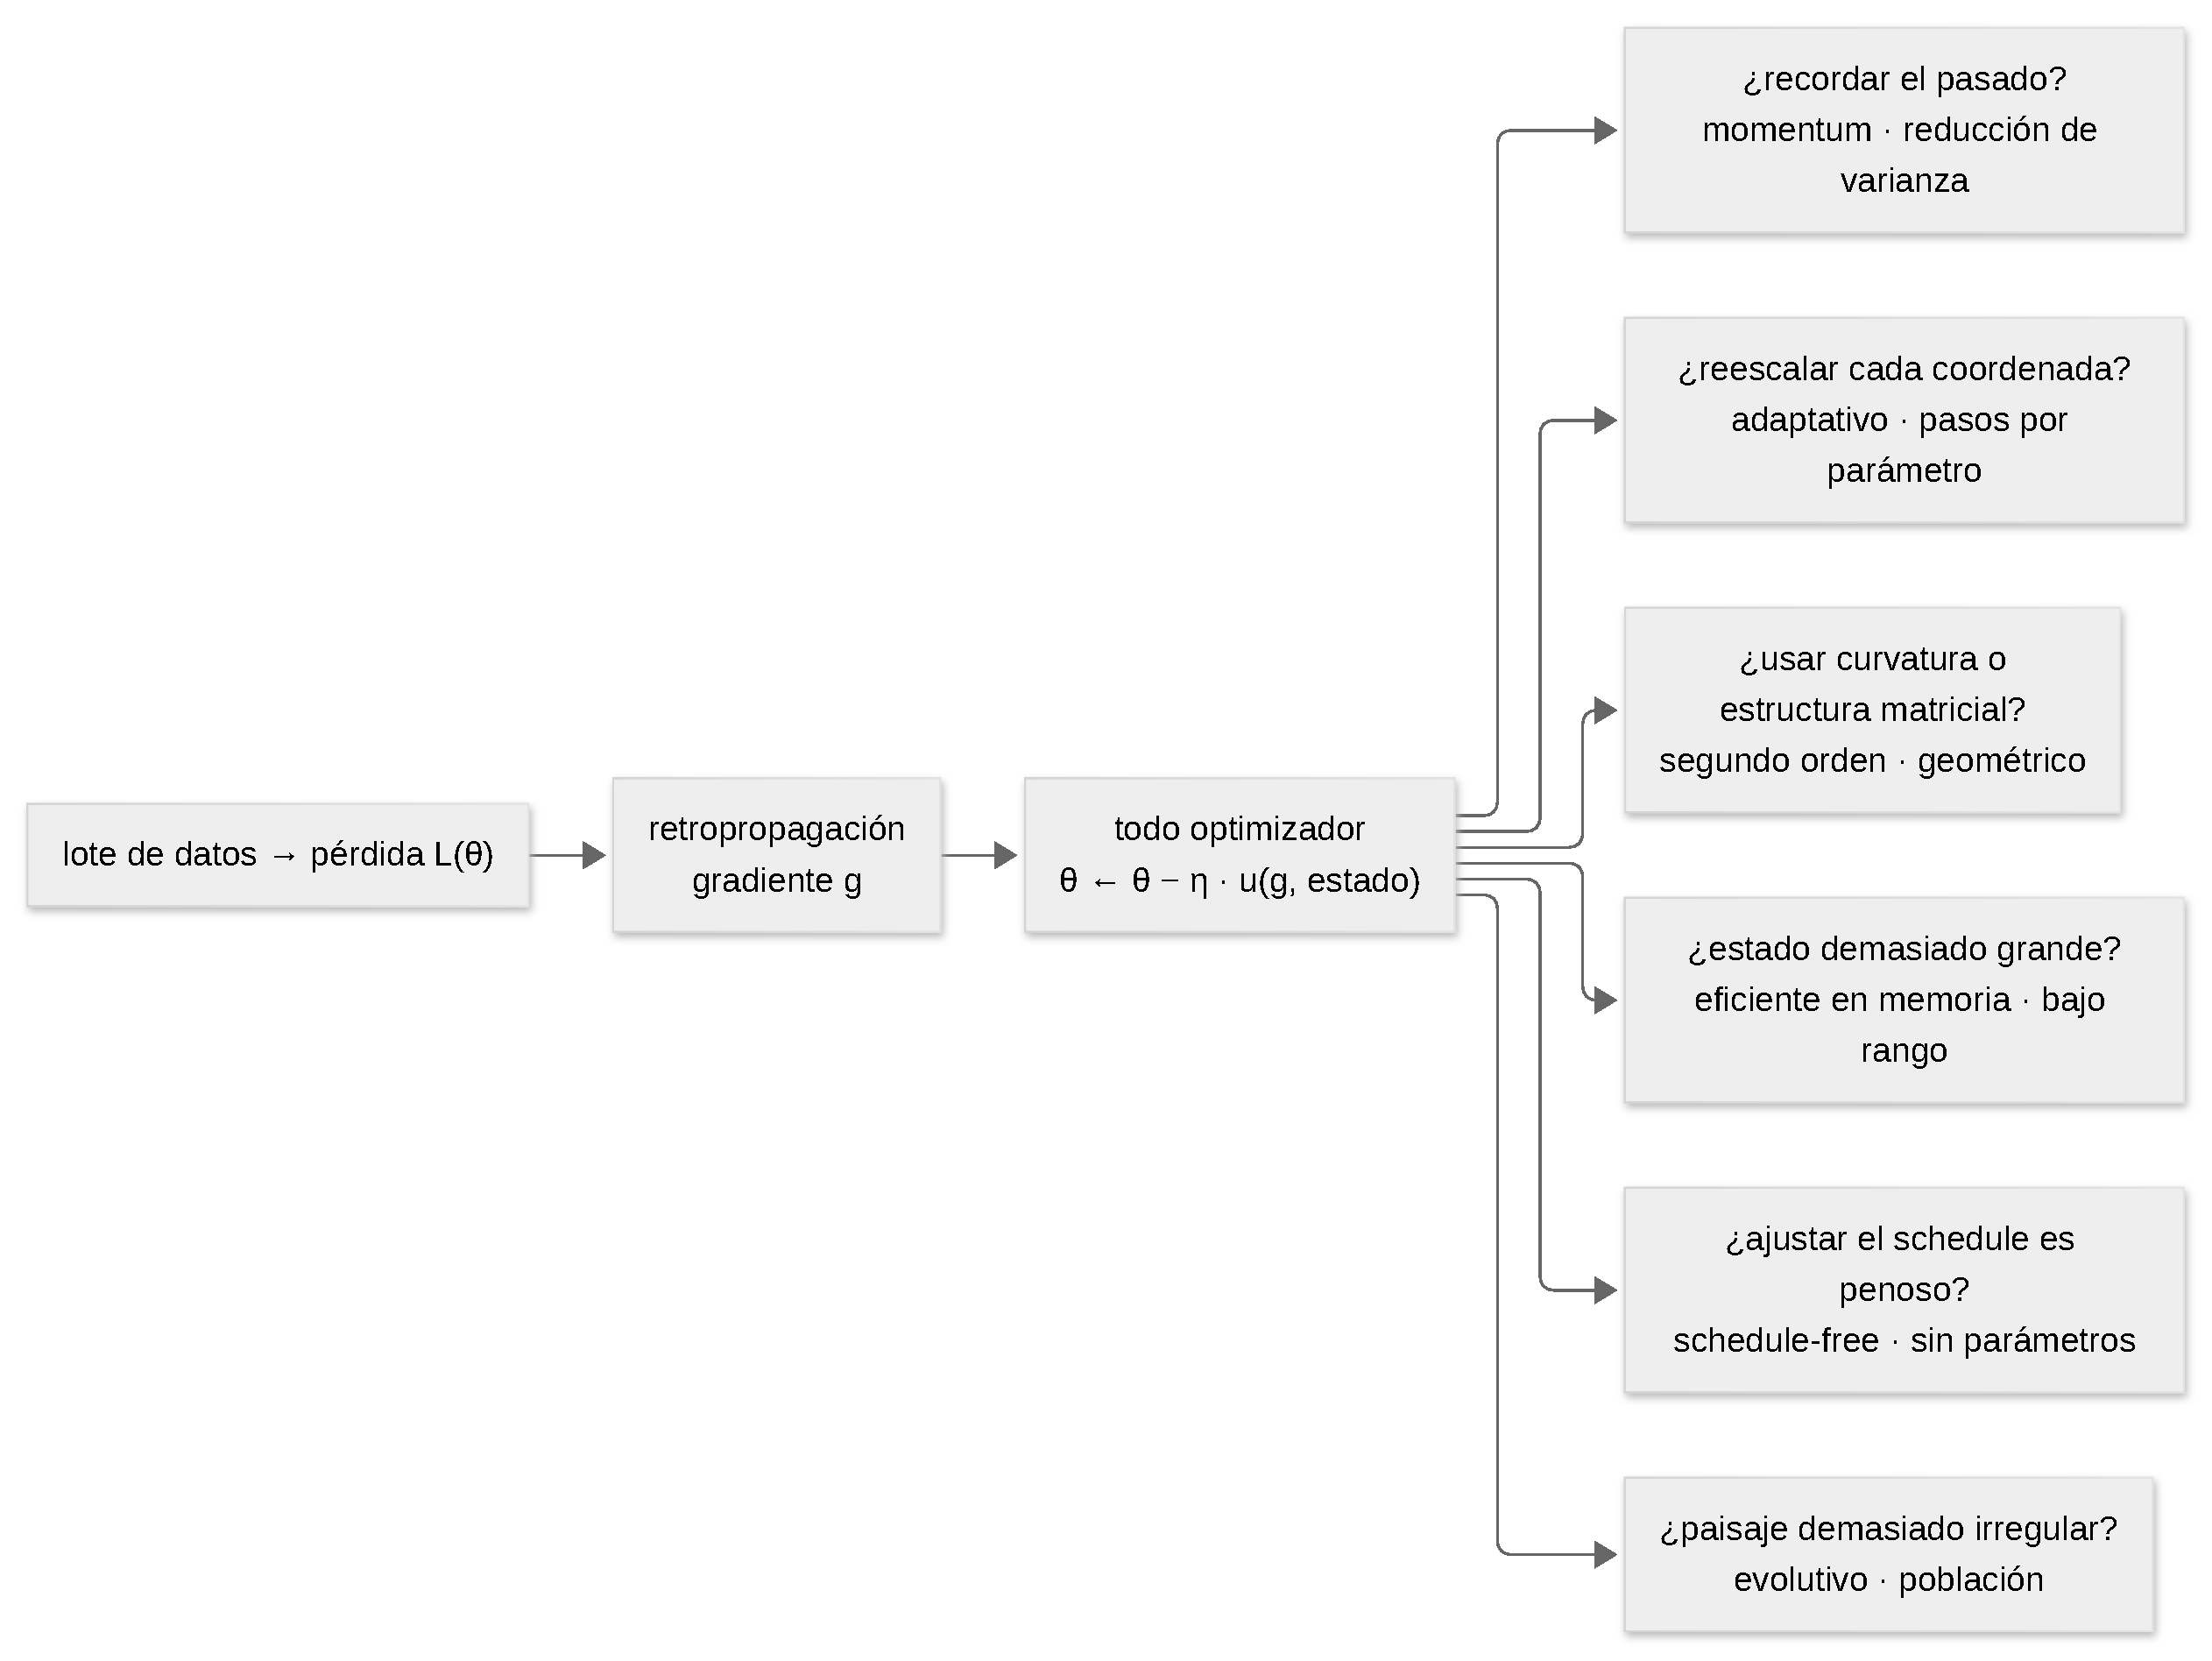
\includegraphics{../paper/figures/optimizer-tutorial-flow-es.pdf}}
\caption{Todo el apéndice en una página. Los datos producen una pérdida, la
retropropagación convierte la pérdida en un gradiente y todo optimizador aplica
la misma regla de actualización con una respuesta distinta a una de seis
preguntas. Las preguntas son independientes, y por eso los métodos se pueden
combinar; también son la única dimensión en la que difieren las familias de la
Sección~\ref{sec:annex-optimizers}.}
\label{fig:opt-tut-flow}
\end{figure}

\subsubsection{Descenso de gradiente: bajar la pendiente}
\label{sec:opt-tutorial-gd}

Para un solo peso $w$, la derivada $f'(w)$ es la pendiente: positiva significa
que la pérdida crece hacia la derecha, de modo que el movimiento útil es hacia
la izquierda. En varias dimensiones el gradiente $\nabla f$ reúne todas las
derivadas parciales y apunta en la dirección de máximo crecimiento; su negativa
es la dirección de máximo descenso. Dar un paso de longitud $\eta$ en ella
produce
\begin{equation}
\theta_{t+1} = \theta_t - \eta\,\nabla f(\theta_t),
\label{eq:opt-tut-gd}
\end{equation}
el algoritmo más antiguo del apéndice, que suele atribuirse a Cauchy en el
siglo XIX y fue analizado por Curry en 1944~\citep{ghojogh_ghodsi_2024}. El
escalar $\eta>0$ es la \emph{tasa de aprendizaje} o tamaño de paso, y es el
único número ajustable.

Dos hechos explican casi todo lo que sigue. Primero, el tamaño de paso tiene un
techo duro. Si el gradiente cambia como mucho $L$ veces más rápido de lo que
cambian los parámetros (el gradiente es \emph{$L$-suave}), entonces
\eqref{eq:opt-tut-gd} disminuye la pérdida para $\eta<2/L$ y diverge más allá;
la elección monótona segura es $\eta\le 1/L$~\citep{ghojogh_ghodsi_2024}.
Segundo, las curvas de nivel de una pérdida cuadrática son elipses cuyos ejes
tienen longitudes muy distintas, y el gradiente negativo es perpendicular a la
curva de nivel pero en general \emph{no} apunta al mínimo---salvo cuando las
elipses son círculos~\citep{hinton_csc321_2012}. El recorrido, por tanto, zigzaguea
a través de la dirección abrupta mientras avanza a rastras por la plana. La
Figura~\ref{fig:opt-tut-gd} muestra los tres regímenes sobre el mismo cuenco, y
la Figura~\ref{fig:opt-tut-lr} muestra cómo se ven como curva de pérdida.

\begin{figure}[H]
\centering
\fitfigure{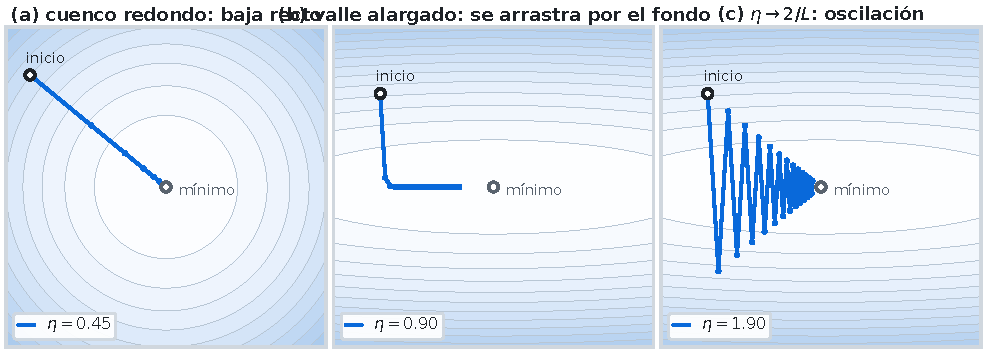
\includegraphics{../paper/figures/optimizers/tutorial/tut-gd-landscape-es.pdf}}
\caption{Descenso de gradiente sobre un cuenco cuadrático, mismo punto de
partida, 26 pasos. (a) Un cuenco isótropo: el gradiente apunta al mínimo y el
recorrido es una línea recta. (b) Un valle cuya curvatura difiere en un factor
veinte entre sus ejes: la dirección abrupta se resuelve en pocos pasos y
después el recorrido avanza a rastras por el fondo, porque el mismo $\eta$ es
demasiado pequeño allí. (c) El mismo valle con $\eta$ empujado hacia el límite
de estabilidad $2/L$: la dirección abrupta alterna de signo y la trayectoria
oscila. Un único tamaño de paso global no puede servir a ambas
direcciones---la observación que motiva todos los métodos por coordenada de
este apéndice~\citep{hinton_csc321_2012}.}
\label{fig:opt-tut-gd}
\end{figure}

\begin{figure}[H]
\centering
\fitfigure{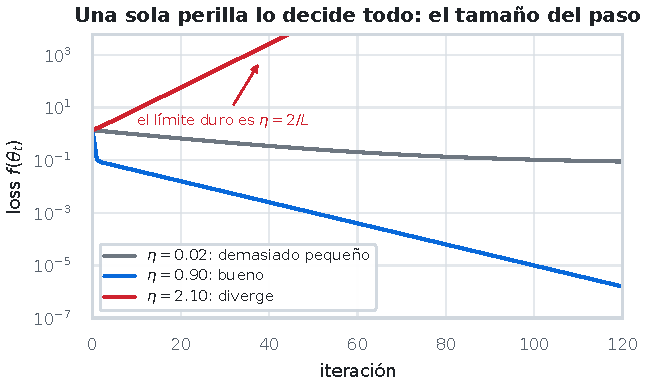
\includegraphics{../paper/figures/optimizers/tutorial/tut-learning-rate-es.pdf}}
\caption{El mismo valle, una sola perilla. Con $\eta$ muy por debajo de $1/L$
la pérdida apenas se mueve; en $\eta\approx1/L$ cae geométricamente; más allá de
$\eta=2/L$ cada iteración multiplica el error por un factor mayor que uno y la
ejecución diverge. Las dos tasas que importan---$1/L$ para un descenso monótono
y $2/L$ para la estabilidad---dependen de la curvatura, que es justo lo que
quien entrena no conoce de antemano.}
\label{fig:opt-tut-lr}
\end{figure}

Cuando la curvatura es desconocida, el remedio clásico es una \emph{búsqueda
lineal}: probar $\eta=1$, dividirlo por dos hasta que la pérdida disminuya de
verdad y repetir~\citep{ghojogh_ghodsi_2024}. El aprendizaje profundo rara vez
lo hace, porque cada prueba cuesta una pasada completa sobre los datos; en su
lugar programa $\eta$ a mano. La teoría proporciona el ritmo: para un objetivo
convexo y $L$-suave, el descenso de gradiente alcanza
$f(\theta_t)-f^\star\le 2L\|\theta_0-\theta^\star\|^2/(t+1)$, es decir,
$O(1/t)$~\citep{ghojogh_ghodsi_2024}. Reducir a la mitad la distancia al óptimo
cuesta duplicar las iteraciones---un resumen justo de por qué los métodos de
primer orden necesitan tantos pasos.

\subsubsection{De dónde sale el gradiente: retropropagación}
\label{sec:opt-tutorial-backprop}

Nada de lo anterior dijo cómo obtener $g_t$. Para una red con millones de pesos
no hay fórmula que derivar a mano, y las diferencias finitas costarían una
pasada hacia adelante por parámetro. La retropropagación calcula todas las
derivadas parciales en un único barrido hacia atrás usando solo la regla de la
cadena.

En una red feed-forward cada capa alterna una aplicación afín y una activación,
$a^{(\ell)}=W^{(\ell)}z^{(\ell-1)}+b^{(\ell)}$ y
$z^{(\ell)}=\sigma(a^{(\ell)})$. La pasada hacia adelante guarda todas las $a$ y
las $z$. La pasada hacia atrás propaga entonces un número por neurona,
$\delta^{(\ell)}=\partial e/\partial a^{(\ell)}$, desde la pérdida hacia la
entrada,
\begin{equation}
\delta^{(L)} = \frac{\partial e}{\partial z^{(L)}}\odot\sigma'(a^{(L)}),
\qquad
\delta^{(\ell)} = \sigma'(a^{(\ell)})\odot
\left(W^{(\ell+1)\top}\delta^{(\ell+1)}\right),
\qquad
\frac{\partial e}{\partial W^{(\ell)}} = \delta^{(\ell)}\,z^{(\ell-1)\top},
\label{eq:opt-tut-backprop}
\end{equation}
donde $\odot$ es el producto elemento a elemento. El gradiente de un peso es,
por tanto, el producto de un número hacia atrás y un número hacia
adelante---las dos cantidades dibujadas en la
Figura~\ref{fig:opt-tut-backprop}. La recursión es lineal en el índice de capa,
así que el barrido completo cuesta aproximadamente lo mismo que una pasada
adicional hacia adelante, en torno al doble del coste de una pasada hacia
adelante por paso, y debe mantener las activaciones de todas las capas en
memoria hasta que se usan~\citep{ghojogh_ghodsi_2024,rumelhart1986learning}.

\begin{figure}[H]
\centering
\fitfigure{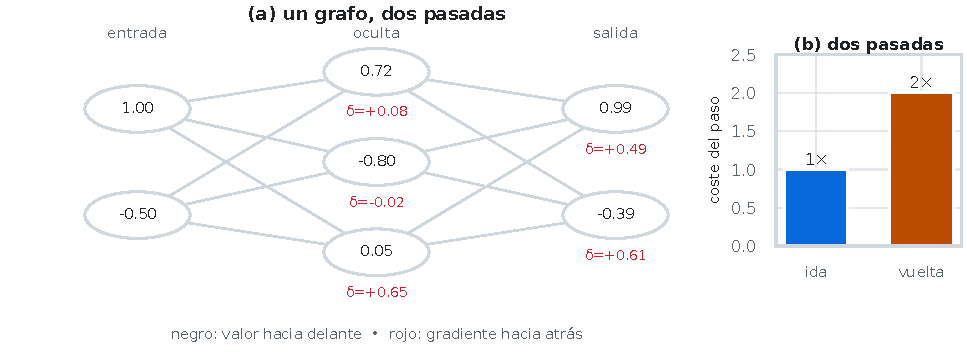
\includegraphics{../paper/figures/optimizers/tutorial/tut-backprop-es.pdf}}
\caption{Un paso de entrenamiento sobre una red con dos capas ocultas y valores
exactos. Los números en negro son las activaciones hacia adelante $z$; los
números en rojo son las cantidades hacia atrás $\delta=\partial e/\partial a$.
Cada gradiente de un peso es el producto de un número rojo y uno negro
(Ecuación~\ref{eq:opt-tut-backprop}), de modo que un solo barrido hacia atrás
los produce todos a la vez. Panel (b): la pasada hacia atrás cuesta alrededor
del doble que la pasada hacia adelante y mantiene vivas las activaciones, y por
eso la memoria del optimizador no es la única factura de memoria del
entrenamiento.}
\label{fig:opt-tut-backprop}
\end{figure}

\begin{algorithm}[H]
\caption{Retropropagación: la fábrica del gradiente}
\label{alg:opt-tut-backprop}
\begin{algorithmic}[1]
\Require Entrada $x$, objetivo $y$, pesos $\{W^{(\ell)},b^{(\ell)}\}_{\ell=1}^{L}$
\Ensure Gradientes $\{\partial e/\partial W^{(\ell)}\}_{\ell=1}^{L}$
\State Hacia adelante: $z^{(0)}\gets x$; \textbf{para} $\ell=1,\dots,L$ \textbf{hacer} $a^{(\ell)}\gets W^{(\ell)}z^{(\ell-1)}+b^{(\ell)}$, $z^{(\ell)}\gets\sigma(a^{(\ell)})$
\State Pérdida: $e \gets \ell(z^{(L)}, y)$
\State $\delta^{(L)} \gets \partial e/\partial z^{(L)} \odot \sigma'(a^{(L)})$
\For{$\ell = L, L-1, \dots, 1$}
    \State $\partial e/\partial W^{(\ell)} \gets \delta^{(\ell)} z^{(\ell-1)\top}$
    \State $\partial e/\partial b^{(\ell)} \gets \delta^{(\ell)}$
    \State $\delta^{(\ell-1)} \gets \sigma'(a^{(\ell-1)})\odot\left(W^{(\ell)\top}\delta^{(\ell)}\right)$
\EndFor
\State \Return todos los gradientes de los pesos
\end{algorithmic}
\end{algorithm}

La consecuencia importante para este apéndice es que la retropropagación no es
un optimizador. Es una fábrica de gradientes, y siempre devuelve el gradiente
exacto del lote que se le entregue. Toda diferencia entre las familias que
siguen vive después de la fábrica, en cómo se forma $u_t$ en
\eqref{eq:opt-tut-generic}.

\subsubsection{Descenso de gradiente estocástico y por mini-lotes}
\label{sec:opt-tutorial-sgd}

Con $n$ ejemplos la pérdida es un promedio, $f(\theta)=\frac1n\sum_i f_i(\theta)$,
así que el gradiente exacto es un promedio de $n$ gradientes por ejemplo y un
paso cuesta $n$ pasadas hacia atrás. Para un conjunto de mil millones de tokens
eso es inasumible, y además derrochador: los ejemplos vecinos suelen decir casi
lo mismo sobre los parámetros.

El descenso de gradiente estocástico, en la línea de la aproximación
estocástica de Robbins--Monro~\citep{robbins_monro_1951}, sustituye el promedio
por un término, $\hat g_t=\nabla f_{i_t}(\theta_t)$ con $i_t$ extraído de forma
uniforme, lo que da
\begin{equation}
\theta_{t+1} = \theta_t - \eta_t\,\nabla f_{i_t}(\theta_t).
\label{eq:opt-tut-sgd}
\end{equation}
La estimación es insesgada, $\mathbb{E}[\hat g_t]=g_t$, así que en promedio
apunta en la dirección correcta; su error cae como $\sigma/\sqrt{b}$ cuando se
usa un lote de $b$ ejemplos en lugar de uno
\citep{ghojogh_ghodsi_2024,bottou_2010}. Las bibliotecas modernas llaman a este
método \emph{por mini-lotes} ``SGD'' y casi nunca usan $b=1$: una pasada sobre
los datos (una \emph{época}) contiene entonces $\lfloor n/b\rfloor$
actualizaciones en lugar de una~\citep{ibm_sgd_2025,ghojogh_ghodsi_2024}. La
Figura~\ref{fig:opt-tut-noise} muestra las dos caras del compromiso: con el
mismo número de pasos y el mismo tamaño de paso, los lotes pequeños vagan, y el
ruido que inyectan es precisamente la cantidad que se reduce como
$1/\sqrt{b}$.

\begin{figure}[H]
\centering
\fitfigure{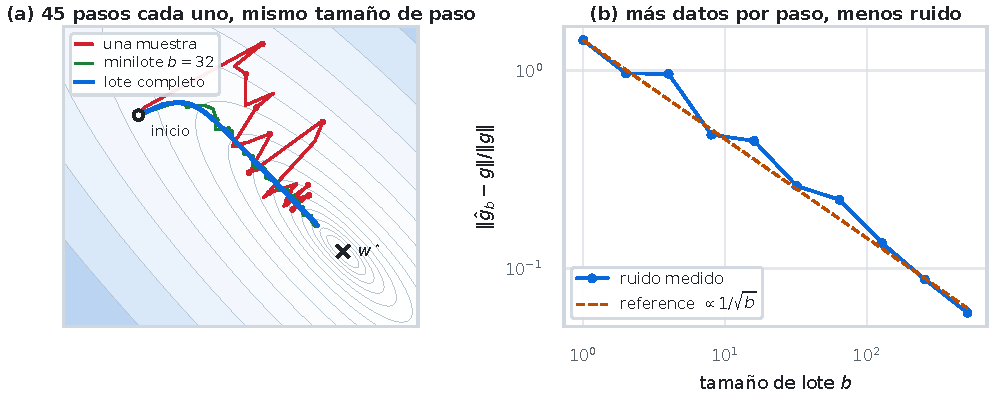
\includegraphics{../paper/figures/optimizers/tutorial/tut-batch-noise-es.pdf}}
\caption{(a) Una superficie de mínimos cuadrados real en dos pesos (rasgos
correlacionados, así que el valle es genuino), con 45 pasos desde el mismo
punto de partida y el mismo tamaño de paso. El lote completo desciende de forma
suave; un mini-lote de 32 lo sigue con un vaivén visible; los gradientes de un
solo ejemplo nunca se asientan. (b) Error relativo del gradiente por lote frente
al gradiente completo, medido sobre los mismos datos: los puntos medidos siguen
la ley $1/\sqrt{b}$, y cuadruplicar el lote reduce el ruido a la mitad.}
\label{fig:opt-tut-noise}
\end{figure}

El ruido no es solo un coste. Como cada paso es una aproximación aleatoria, el
iterado puede abandonar una cuenca poco profunda o deslizarse por un punto de
silla que un método de lote completo trataría como punto de
parada~\citep{ibm_sgd_2025}. El precio aparece en la tasa. Para un objetivo
convexo y $L$-suave, SGD con $\eta_t\propto1/\sqrt t$ satisface
$f(\theta_t)-f^\star=O(\log t/\sqrt t)$, y con un paso constante converge a un
entorno de tamaño $O(\eta)$ y luego se
estanca~\citep{ghojogh_ghodsi_2024}. El descenso de gradiente con lote completo
es, por tanto, más preciso por iteración y mucho más lento por iteración; SGD
es lo contrario. La Figura~\ref{fig:opt-tut-rates} pone ambas afirmaciones sobre
los mismos ejes, una vez por iteración y otra por unidad de tiempo de reloj, que
es la comparación que de verdad importa cuando un paso cuesta $n/b$ veces menos.

\begin{figure}[H]
\centering
\fitfigure{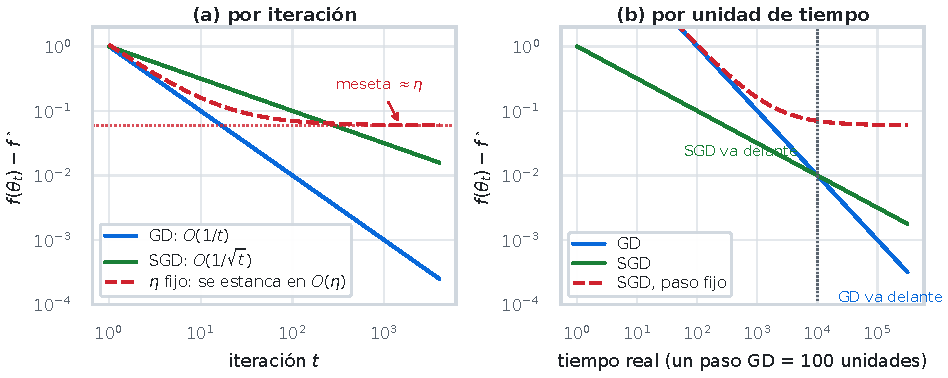
\includegraphics{../paper/figures/optimizers/tutorial/tut-convergence-es.pdf}}
\caption{(a) Por iteración, el descenso de gradiente decae como $O(1/t)$
mientras que SGD decae como $O(1/\sqrt t)$ y, con un paso fijo, se aplana en una
meseta de altura $O(\eta)$~\citep{ghojogh_ghodsi_2024}. La meseta es la razón por
la que toda receta práctica acaba reduciendo $\eta$. (b) Las mismas curvas frente
al tiempo de reloj, con un paso de lote completo costando cien pasos de
mini-lote: SGD va por delante durante la mayor parte de la ejecución y el
descenso de gradiente solo gana cuando la meseta manda. Las curvas son
esquemáticas, con constantes elegidas para facilitar la lectura.}
\label{fig:opt-tut-rates}
\end{figure}

\subsubsection{Dos perillas que giran todos los métodos posteriores}
\label{sec:opt-tutorial-knobs}

Todo lo que sigue es un refinamiento de dos observaciones sobre la
Ecuación~\eqref{eq:opt-tut-gd}, y merece la pena separarlas antes de conocer las
familias.

\paragraph{Memoria del pasado.} Una bola que rueda por el mismo valle conserva
su velocidad: acumula rapidez a lo largo de una pendiente constante y cancela la
oscilación cuando la pendiente cambia de signo continuamente. Momentum
implementa exactamente eso, sustituyendo el gradiente por una suma decreciente
de gradientes,
\begin{equation}
v_t = \beta\,v_{t-1} - \eta\,g_t,
\qquad
\theta_{t+1} = \theta_t + v_t,
\label{eq:opt-tut-momentum}
\end{equation}
con $\beta\in[0,1)$ el decaimiento. El paso efectivo es $\eta/(1-\beta)$ a lo
largo de una dirección estable, que es como un $\eta$ pequeño puede aun así
moverse deprisa. Momentum de Nesterov hace el mismo movimiento pero lee el
gradiente en la posición hacia la que se dirige la velocidad, de modo que la
corrección llega antes que el sobrepaso~\citep{hinton_csc321_2012,sutskever2013importance}.
La Figura~\ref{fig:opt-tut-momentum} muestra la composición de los dos términos
y su efecto sobre el valle.

\begin{figure}[H]
\centering
\fitfigure{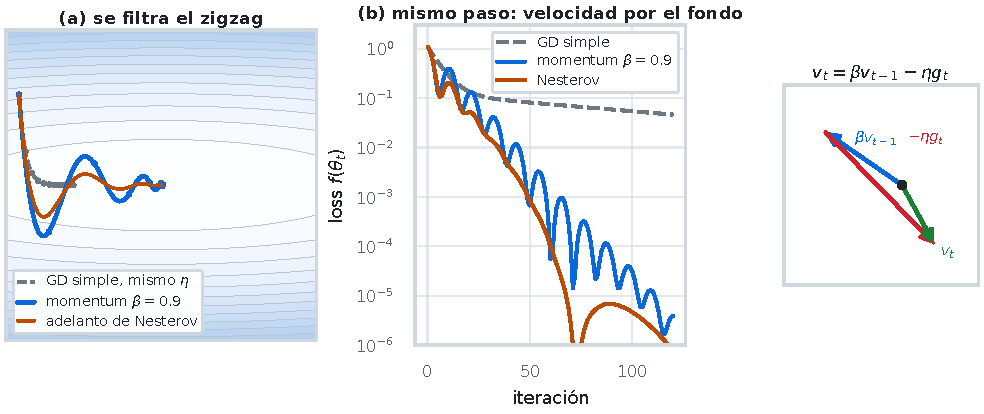
\includegraphics{../paper/figures/optimizers/tutorial/tut-momentum-es.pdf}}
\caption{Momentum como memoria. (a) Sobre el valle de la
Figura~\ref{fig:opt-tut-gd}(b), con el mismo tamaño de paso, el descenso de
gradiente simple sigue avanzando a rastras por el fondo tras 120 pasos mientras
que momentum y su variante de Nesterov alcanzan el mínimo. (b) La misma
ejecución como curva de pérdida: la dirección recordada compra aproximadamente
un orden de magnitud. (c) La actualización es la suma cabeza-cola de la velocidad
amortiguada (azul) y el paso fresco del gradiente (rojo); el resultado (verde) es
más suave que cualquiera de los dos términos por separado.}
\label{fig:opt-tut-momentum}
\end{figure}

\paragraph{Un tamaño de paso por coordenada.} La segunda observación es que el
valle de la Figura~\ref{fig:opt-tut-gd}(b) no tiene un $\eta$ bueno único: lo que
es estable a lo largo del eje abrupto es despreciable a lo largo del plano. Los
métodos adaptativos mantienen un promedio móvil de gradientes al cuadrado y
dividen por su raíz cuadrada, de modo que una coordenada que ha recibido
gradientes grandes recibe un paso menor y una coordenada tranquila recibe uno
mayor,
\begin{equation}
s_t = \gamma\,s_{t-1} + (1-\gamma)\,g_t^2,
\qquad
\theta_{t+1} = \theta_t - \eta\,\frac{g_t}{\sqrt{s_t}+\epsilon}.
\label{eq:opt-tut-rms}
\end{equation}
El esquema nació de rprop, que usaba solo el signo del gradiente, y de su versión
por mini-lotes, rmsprop~\citep{hinton_csc321_2012,tieleman_hinton2012}; AdaGrad es
la versión acumulativa en lugar de decreciente~\citep{duchi_adagrad_2011}. La
Figura~\ref{fig:opt-tut-adaptive} muestra el efecto: los dos ejes del valle
reciben desplazamientos comparables, a cambio de un estado por coordenada y de
un paso que ya no se reduce por sí solo---el temblor residual de tamaño
$\approx\eta$ alrededor del mínimo es lo que después motiva tamaños de paso
decrecientes o sin programación.

\begin{figure}[H]
\centering
\fitfigure{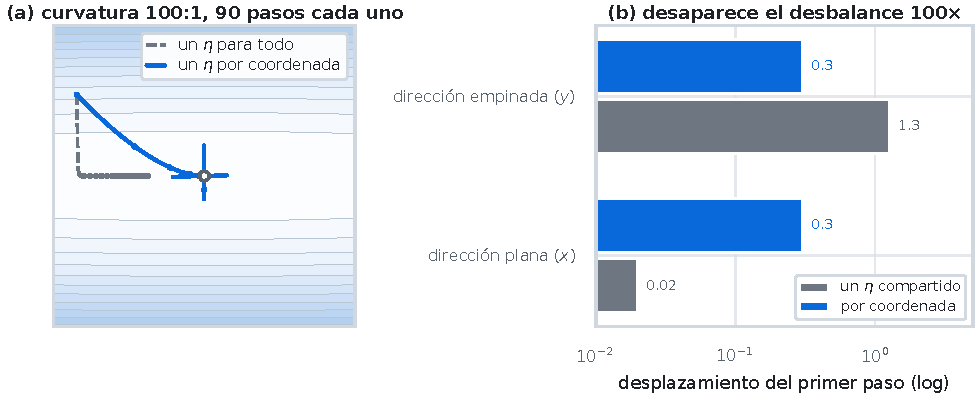
\includegraphics{../paper/figures/optimizers/tutorial/tut-adaptive-es.pdf}}
\caption{Un tamaño de paso por coordenada. (a) Sobre un valle con una razón de
curvatura de cien a uno, un tamaño de paso compartido o sobrepasa el eje abrupto
o ignora el plano; normalizar cada coordenada por la raíz del promedio de sus
gradientes recientes alcanza la cuenca y tiembla a su alrededor. (b) Desplazamiento
del primer paso por coordenada, en eje logarítmico: el paso compartido produce un
factor sesenta entre los ejes, el normalizado no produce ninguno.}
\label{fig:opt-tut-adaptive}
\end{figure}

Las dos perillas se componen, y su composición es la razón por la que AdamW es
el valor por defecto en la práctica: un primer momento para la dirección, un
segundo momento para la escala, una corrección de sesgo para los primeros pasos
vacíos y un decaimiento de pesos desacoplado para la
regularización~\citep{kingma_adam_2014}. Nada en las
Ecuaciones~\eqref{eq:opt-tut-momentum} y~\eqref{eq:opt-tut-rms} es específico de
los transformers; lo que difiere entre familias es qué estadísticos se guardan,
cómo se combinan y cuántos bytes por parámetro cuesta. Una panorámica compacta
del zoo resultante la ofrece \citet{ruder_2016}.

\subsubsection{En qué difieren las familias}
\label{sec:opt-tutorial-families}

El apéndice que sigue contiene treinta y ocho métodos, demasiados para
retenerlos a la vez. Se recuerdan mejor como ocho familias, cada una respondiendo
a una de las preguntas de la Figura~\ref{fig:opt-tut-flow} y cada una distinguida
por lo que recuerda y lo que paga.

\begin{itemize}[leftmargin=*]
\item \textbf{Líneas base de primer orden} (SGD con momentum, AdamW, RAdam)
guardan uno o dos estadísticos por parámetro y suponen que el paisaje es lo
bastante suave para un modelo localmente lineal. Son la referencia contra la que
se mide todo lo demás.
\item \textbf{Momentum y reducción de varianza} (Adan, ADOPT, AdEMAMix, MARS,
Cautious AdamW) guardan más de dos búferes, o una diferencia de gradientes, para
reducir la varianza de la propia actualización. Compran estabilidad y velocidad a
cambio de memoria y de una segunda evaluación del gradiente o de un historial más
largo.
\item \textbf{Eficientes en memoria y de rango bajo} (Adafactor, GaLore, APOLLO,
Lion, AdamPM) aceptan una peor estimación del segundo momento---factorizada,
proyectada o inexistente---precisamente para encoger el estado. Lion llega a
guardar solo el signo de la actualización.
\item \textbf{Sin programación y sin parámetros} (Schedule-Free AdamW, Prodigy,
LAMB para lotes grandes) trasladan la carga de elegir $\eta_t$ de quien entrena
al algoritmo, normalmente promediando iterados o estimando el paso a partir de la
propia pérdida.
\item \textbf{Curvatura y segundo orden} (Sophia, Shampoo, SOAP) estiman cómo
cambia el gradiente, no solo su tamaño, y precondicionan el paso con esa
estimación. Convergen en menos iteraciones y cuestan más por iteración.
\item \textbf{Geométricos y de ortogonalidad} (Muon, Turbo-Muon, AF-Muon, ROOT,
NorMuon, Dion3) tratan una matriz de pesos como una matriz: ortogonalizan o
blanquean la actualización para que todas las direcciones singulares avancen a la
misma tasa, que es un sustituto barato de la curvatura en parámetros con forma de
matriz.
\item \textbf{Adaptividad ajustable} (Anon) mantiene el estado estándar pero
adapta sus propios coeficientes, de modo que la cantidad de adaptividad es un
hiperparámetro y no una decisión de diseño fija.
\item \textbf{Evolutivos y de población} (EvE, EA4LLM) no siguen ningún gradiente:
muestrean perturbaciones o mantienen una población de modelos, lo que resulta
atractivo cuando los gradientes son ruidosos, no están disponibles o hay que
ajustar muchos hiperparámetros a la vez, y caro cuando el modelo es grande.
\end{itemize}

El Cuadro~\ref{tab:opt-tut-families} expresa la misma comparación en las dos
monedas que deciden una ejecución real: qué se almacena por parámetro y cuánto
cuesta cada paso. La Figura~\ref{fig:opt-tut-families} lo convierte en una huella:
leer hacia abajo una fila dice qué ingredientes usa una familia, y leer a través
de una columna dice qué familias comparten uno.

\begin{table}[H]
\centering
\caption{Las ocho familias por la pregunta que responden y lo que cuestan. El
estado es aproximado, en flotantes por parámetro; $k$ es un rango o un número de
bloques y $P$ un tamaño de población. Ninguna familia es uniformemente mejor:
cada línea es un compromiso.}
\label{tab:opt-tut-families}
\small
\begin{tabular}{@{}L{3.2cm}L{4.6cm}L{2.6cm}L{4.6cm}@{}}
\toprule
Familia & Pregunta que responde & Estado por parámetro & Riesgo principal \\
\midrule
Primer orden & ¿Cuál es la pendiente? & 0--2 & exige programar la tasa \\
Momentum, varianza & ¿Hacia dónde va? & 2--3 & más memoria y contabilidad \\
Memoria, rango bajo & ¿Cabe en menos estado? & $\le1$ & segundo momento sesgado \\
Sin programación & ¿Se elige $\eta_t$ por mí? & 1 & la teoría supone convexidad \\
Curvatura, 2.\textsuperscript{o} orden & ¿Cómo cambia la pendiente? & $2+2k$ & factorizaciones caras \\
Geométricos, ortogonalidad & ¿Tiene buena forma el paso? & 1 & solo matrices \\
Adaptividad ajustable & ¿Cuánta adaptividad? & 2 & hiperparámetros extra \\
Evolutivos, población & ¿Sin gradientes? & $P\times$ & prohibitivo a escala \\
\bottomrule
\end{tabular}
\end{table}

\begin{figure}[H]
\centering
\fitfigure{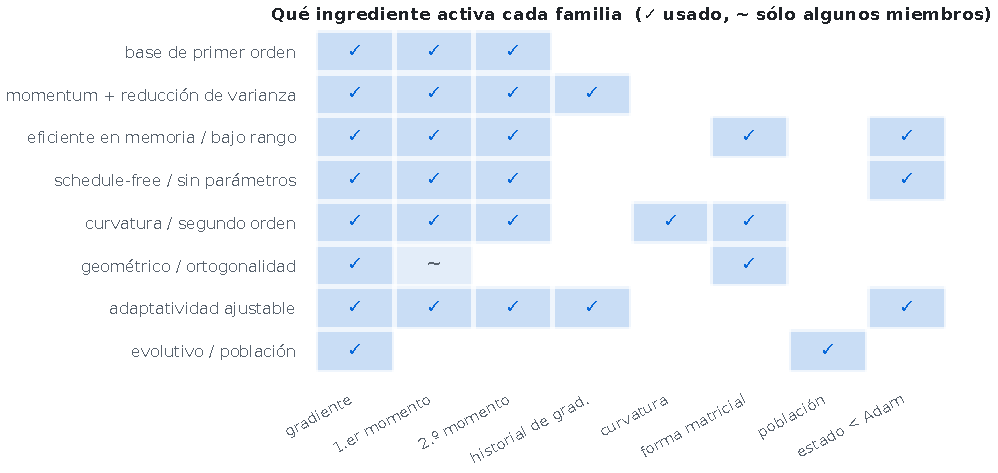
\includegraphics{../paper/figures/optimizers/tutorial/tut-families-es.pdf}}
\caption{Huella de las ocho familias. Una marca indica un ingrediente que la
familia usa y una tilde uno que solo usan algunos miembros. La primera columna
está marcada en todas partes---toda familia de este apéndice es un método de
gradiente salvo la última---y las columnas restantes son los ejes reales de
variación: memoria de dirección, escala por coordenada, curvatura, estructura
matricial, población y un estado menor que el de Adam. El mapa es deliberadamente
grueso; las entradas que siguen dan las reglas exactas.}
\label{fig:opt-tut-families}
\end{figure}

El Algoritmo~\ref{alg:opt-tut-generic} hace operativa la comparación: las
familias difieren solo en qué ranuras rellenan. Leerlo junto al
Cuadro~\ref{tab:opt-tut-knobs} basta para situar cualquier método del resto del
apéndice sin memorizar su álgebra.

\begin{algorithm}[H]
\caption{Cualquier optimizador de este apéndice, con las ranuras específicas de
familia abiertas}
\label{alg:opt-tut-generic}
\begin{algorithmic}[1]
\Require Parámetros $\theta_0$, tasa $\eta$, ranuras
$\mathcal{S}$ (estado), $\mathcal{D}$ (dirección), $\mathcal{P}$ (precondicionador), $\mathcal{T}$ (regla de paso)
\Ensure Parámetros actualizados $\theta_T$
\State Inicializar el estado que requiere $\mathcal{S}$
\For{$t = 1, 2, \ldots, T$}
    \State Muestrear un lote $\mathcal{B}_t$ y calcular $g_t\gets\nabla f_{\mathcal{B}_t}(\theta_{t-1})$ \Comment{retropropagación}
    \State Actualizar el estado: $\mathcal{S}\gets\textsc{Actualizar}(\mathcal{S}, g_t, \theta_{t-1})$ \Comment{1.\textsuperscript{er}/2.\textsuperscript{o} momento, curvatura, población}
    \State Formar la dirección $u_t\gets\mathcal{D}(g_t,\mathcal{S})$ \Comment{gradiente crudo, momentum, signo, ortogonalizado}
    \State Aplicar el precondicionador $u_t\gets\mathcal{P}(u_t,\mathcal{S})$ \Comment{escala por coordenada, factorizada o completa}
    \State Elegir el paso $\eta_t\gets\mathcal{T}(\eta, t, \mathcal{S})$ \Comment{constante, programado, implícito, autoajustado}
    \State $\theta_t\gets\theta_{t-1}-\eta_t\,u_t$ \Comment{opcionalmente tras decaimiento desacoplado}
\EndFor
\State \Return $\theta_T$
\end{algorithmic}
\end{algorithm}

\begin{table}[H]
\centering
\caption{Las ranuras del Algoritmo~\ref{alg:opt-tut-generic} y la perilla que
gira cada una. Un método se identifica por las ranuras que rellena, no por su
nombre.}
\label{tab:opt-tut-knobs}
\small
\begin{tabular}{@{}L{2.4cm}L{4.4cm}L{3.4cm}L{3.6cm}@{}}
\toprule
Ranura & Qué decide & Perilla girada & Se ve en \\
\midrule
$\mathcal{B}_t$ & cuántos ejemplos por paso & varianza & SGD, mini-lote, lote completo \\
$\mathcal{S}$ & qué se recuerda & estado y memoria & momentum, Adam, Sophia, Shampoo \\
$\mathcal{D}$ & qué dirección se sigue & suavizado & momentum, Nesterov, métodos de signo \\
$\mathcal{P}$ & cómo se reescalan las coordenadas & acondicionamiento & AdaGrad, RMSProp, Adam, Muon \\
$\mathcal{T}$ & cuánto mide el paso & programación & coseno, calentamiento, sin programación, Prodigy \\
decaimiento & cómo se regularizan los pesos & generalización & L2, decaimiento desacoplado \\
\bottomrule
\end{tabular}
\end{table}

\subsubsection{Leer una curva de pérdida}
\label{sec:opt-tutorial-diagnostics}

El valor práctico de las cinco ideas es diagnóstico. Una sola curva de pérdida
ya dice cuál de ellas está mal, y la respuesta suele ser visible en unos cientos
de pasos (Figura~\ref{fig:opt-tut-diag}).

\begin{figure}[H]
\centering
\fitfigure{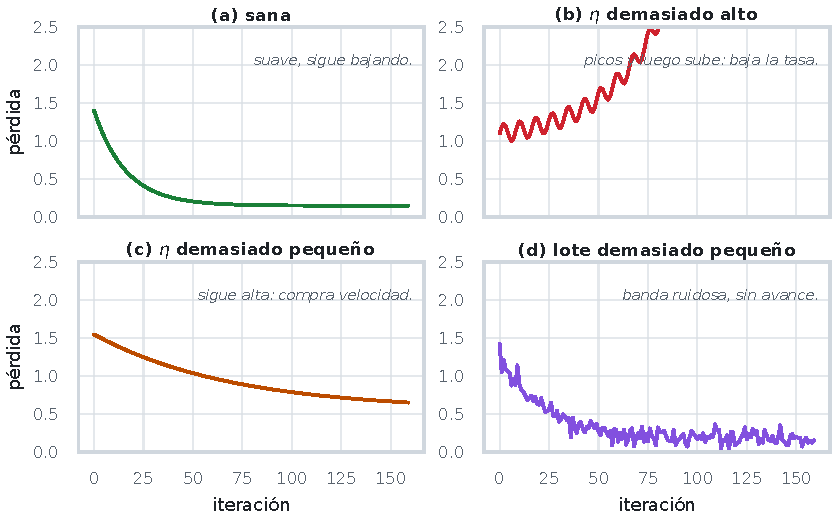
\includegraphics{../paper/figures/optimizers/tutorial/tut-loss-diagnostics-es.pdf}}
\caption{Cuatro curvas de pérdida y la frase que pronuncia cada una. Una curva
suave que sigue bajando es sana; los picos seguidos de una subida significan que
el tamaño de paso cruzó $2/L$; una curva suave pero demasiado alta significa que
el tamaño de paso está muy por debajo de $1/L$ o que la programación decayó
demasiado pronto; una curva que alcanza una banda ruidosa y deja de mejorar suele
significar que el lote es demasiado pequeño o que el paso ha llegado a su meseta
$O(\eta)$.}
\label{fig:opt-tut-diag}
\end{figure}

Cinco reglas prácticas cierran el tutorial, todas consecuencias de las figuras
anteriores y no de ningún método concreto.
\begin{enumerate}[leftmargin=*]
\item Empezar por una línea base de primer orden con ambos momentos (AdamW). Es
la configuración más barata que sobrevive a curvatura heterogénea.
\item Si el estado del optimizador no cabe en memoria, cambiar de familia antes
que de hiperparámetros: las familias eficientes en memoria y de rango bajo
existen exactamente para esa restricción.
\item Si programar la tasa consume el presupuesto experimental, las familias sin
programación y sin parámetros eliminan la perilla en lugar de ajustarla.
\item Si la mayoría de los parámetros viven en matrices (proyecciones de atención
y feed-forward), los métodos geométricos explotan una estructura que los métodos
elemento a elemento ignoran; si el modelo es pequeño y la búsqueda abarca muchas
configuraciones, los métodos de población se vuelven asequibles.
\item Cambiar una ranura a la vez. Como las familias son composiciones
ortogonales, una ejecución que cambia dos de ellas no puede atribuir su resultado.
\end{enumerate}

El resto de este apéndice es la referencia detrás de estas afirmaciones: una
entrada por método, cada una indicando su regla de actualización, su
pseudocódigo, su perfil de memoria y el compromiso que asume.
